\section{Geometric interpretation of eigenvectors}

Consider the matrix
\begin{equation*}
  A = \begin{mymatrix}{rr}
    2 & 1 \\
    1 & 2 \\
  \end{mymatrix}.
\end{equation*}
In Chapter~\ref{cha:linear-transformation}, we saw that this matrix
corresponds to a linear transformation $T : \R^2\to\R^2$ defined by
$T(\vect{x}) = A\vect{x}$. We also saw how to visualize this linear
transformation as a before-and-after picture. For this, we
considered the images of the first and second standard basis vectors,
which are the first and second column of $A$:
\begin{align*}
  T(\vect{e}_1) &= A\vect{e}_1 = \begin{mymatrix}{r} 2 \\ 1 \end{mymatrix},\\
  T(\vect{e}_2) &= A\vect{e}_2 = \begin{mymatrix}{r} 1 \\ 2 \end{mymatrix}.
\end{align*}
Here is the before-and-after picture for this transformation:
\vspace{-2cm}
\begin{center}
  \begin{tikzpicture}
    \begin{scope}[scale=0.4]
      \draw[red,thick,fill=red!15]
      (0,0) -- (0,5) -- (3,5) -- (3,4) -- (1,4) --
      (1,3) -- (2,3) -- (2,2) -- (1,2) -- (1,0) -- cycle;
      \draw[step=1cm, gray!50, very thin] (-5.8,-5.8) grid (5.8,5.8);
      \draw[red,thick]
      (0,0) -- (0,5) -- (3,5) -- (3,4) -- (1,4) --
      (1,3) -- (2,3) -- (2,2) -- (1,2) -- (1,0) -- cycle;
      \draw[semithick,->] (-6.5,0) -- (6.5,0);
      \draw[semithick,->] (0,-6.5) -- (0,6.5);
      \draw[blue,thick,->] (0,0) -- node[below] {$\vect{e}_1$} (5,0);
      \draw[blue,thick,->] (0,0) -- node[left] {$\vect{e}_2$} (0,5);
    \end{scope}
    \begin{scope}[xshift=3.6cm]
      \path (0,0) node {$\stackrel{T}{\longmapsto}$};
    \end{scope}
    \begin{scope}[xshift=7.2cm,scale=0.4]
      \draw[red,thick,fill=red!15,cm={2,1,1,2,(0,0)}]
      (0,0) -- (0,5) -- (3,5) -- (3,4) -- (1,4) --
      (1,3) -- (2,3) -- (2,2) -- (1,2) -- (1,0) -- cycle;
      \draw[step=1cm, gray!50, very thin] (-5.8,-5.8) grid (5.8,5.8);
      \draw[red,thick,cm={2,1,1,2,(0,0)}]
      (0,0) -- (0,5) -- (3,5) -- (3,4) -- (1,4) --
      (1,3) -- (2,3) -- (2,2) -- (1,2) -- (1,0) -- cycle;
      \draw[semithick,->] (-6.5,0) -- (6.5,0);
      \draw[semithick,->] (0,-6.5) -- (0,6.5);
      \draw[blue,thick,->,cm={2,1,1,2,(0,0)}] (0,0) --
      node[below right]
      {$T(\vect{e}_1) = \begin{mysmallmatrix}{r}2\\1\end{mysmallmatrix}$}
      (5,0);
      \draw[blue,thick,->,cm={2,1,1,2,(0,0)}] (0,0) --
      node[left,xshift=-0.1cm,pos=0.8]
      {$T(\vect{e}_2) = \begin{mysmallmatrix}{c}1\\2\end{mysmallmatrix}$}
      (0,5);
    \end{scope}
  \end{tikzpicture}
\end{center}
Although we can see from this picture that the letter ``F'' is being
distorted somehow, it is not so very obvious what exactly this linear
transformation is doing.

Now let us compute the eigenvectors and eigenvalues of $A$. A short
calculation shows that the basic eigenvectors are
\begin{equation*}
  \vect{v}_1 = \begin{mymatrix}{r} 1 \\ 1 \end{mymatrix}
  \quad\mbox{and}\quad
  \vect{v}_2 = \begin{mymatrix}{r} -1 \\ 1 \end{mymatrix},
\end{equation*}
with corresponding eigenvalues $\lambda_1=3$ and $\lambda_2=1$.
Consider the effect of the linear transformation $T$ on the
eigenvectors:
\begin{align*}
  T(\vect{v}_1) &= \begin{mymatrix}{rr}
    2 & 1 \\
    1 & 2 \\
  \end{mymatrix} \begin{mymatrix}{r} 1 \\ 1 \end{mymatrix}
  = \begin{mymatrix}{r} 3 \\ 3 \end{mymatrix}
  = 3\vect{v}_1, \\
  T(\vect{v}_2) &= \begin{mymatrix}{rr}
    2 & 1 \\
    1 & 2 \\
  \end{mymatrix} \begin{mymatrix}{r} -1 \\ 1 \end{mymatrix}
  = \begin{mymatrix}{r} -1 \\ 1 \end{mymatrix}
  = \vect{v}_2.
\end{align*}
So each eigenvector is mapped to a scalar multiple of itself. This
gives us a hint for how to draw a more useful before-and-after
picture. Rather than tracking the movement of the standard basis
vectors $\vect{e}_1$ and $\vec{e}_2$, let us track the movement of the
eigenvectors $\vect{v}_1$ and $\vect{v}_2$ instead:
\begin{center}
  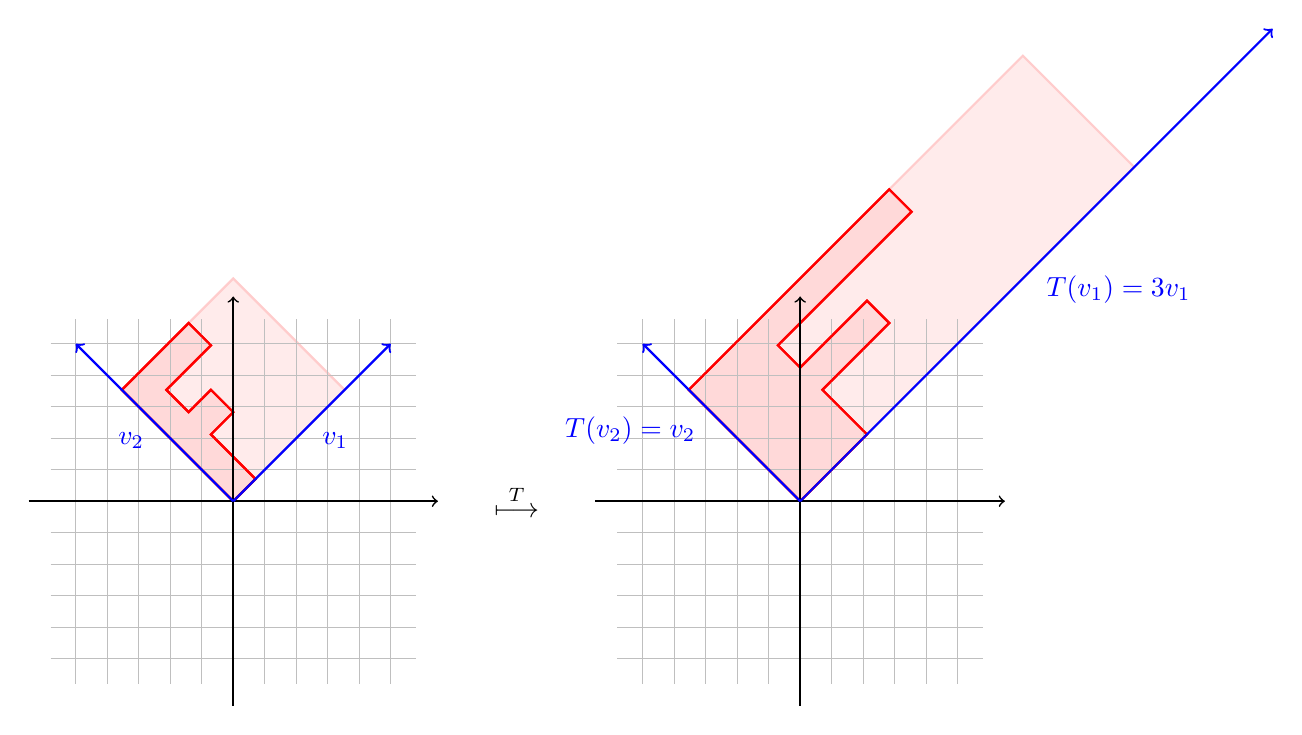
\begin{tikzpicture}
    \begin{scope}[scale=0.4]
      \draw[red!20,thick,fill=red!8,rotate=45]
      (0,0) -- (0,5) -- (5,5) -- (5,0) -- cycle;
      \draw[red,thick,fill=red!15,rotate=45]
      (0,0) -- (0,5) -- (3,5) -- (3,4) -- (1,4) --
      (1,3) -- (2,3) -- (2,2) -- (1,2) -- (1,0) -- cycle;
      \draw[step=1cm, gray!50, very thin] (-5.8,-5.8) grid (5.8,5.8);
      \draw[red,thick,rotate=45]
      (0,0) -- (0,5) -- (3,5) -- (3,4) -- (1,4) --
      (1,3) -- (2,3) -- (2,2) -- (1,2) -- (1,0) -- cycle;
      \draw[semithick,->] (-6.5,0) -- (6.5,0);
      \draw[semithick,->] (0,-6.5) -- (0,6.5);
      \draw[blue,thick,->] (0,0) -- node[below right] {$\vect{v}_1$} (5,5);
      \draw[blue,thick,->] (0,0) -- node[below left] {$\vect{v}_2$} (-5,5);
    \end{scope}
    \begin{scope}[xshift=3.6cm]
      \path (0,0) node {$\stackrel{T}{\longmapsto}$};
    \end{scope}
    \begin{scope}[xshift=7.2cm,scale=0.4]
      \draw[red!20,thick,fill=red!8,rotate=45,xscale=3]
      (0,0) -- (0,5) -- (5,5) -- (5,0) -- cycle;
      \draw[red,thick,fill=red!15,rotate=45,xscale=3]
      (0,0) -- (0,5) -- (3,5) -- (3,4) -- (1,4) --
      (1,3) -- (2,3) -- (2,2) -- (1,2) -- (1,0) -- cycle;
      \draw[step=1cm, gray!50, very thin] (-5.8,-5.8) grid (5.8,5.8);
      \draw[red,thick,rotate=45,xscale=3]
      (0,0) -- (0,5) -- (3,5) -- (3,4) -- (1,4) --
      (1,3) -- (2,3) -- (2,2) -- (1,2) -- (1,0) -- cycle;
      \draw[semithick,->] (-6.5,0) -- (6.5,0);
      \draw[semithick,->] (0,-6.5) -- (0,6.5);
      \draw[blue,thick,->,cm={2,1,1,2,(0,0)}] (0,0) --
      node[below right]
      {$T(\vect{v}_1) = 3\vect{v}_1$}
      (5,5);
      \draw[blue,thick,->,cm={2,1,1,2,(0,0)}] (0,0) --
      node[below left,pos=0.6]
      {$T(\vect{v}_2) = \vect{v}_2$}
      (-5,5);
    \end{scope}
  \end{tikzpicture}
\end{center}
Thus, the linear transformation described by the matrix $A$ is
revealed to be just a scaling by a factor of $3$ along the direction of
\begin{equation*}
  \vect{v}_1 = \begin{mymatrix}{r} 1 \\ 1 \end{mymatrix}.
\end{equation*}
In summary, the geometric meaning of an eigenvector is that it is
mapped to a multiple of itself. Thus, when viewed from the point of
view of its eigenvectors, a linear transformation behaves like a
scaling, with each eigenvector giving a direction of scaling, and each
corresponding eigenvalue giving the corresponding scaling factor.

\begin{example}
  Visualize the linear transformation $T:\R^2\to\R^2$ that is
  described by the matrix
  \begin{equation*}
    A = \begin{mymatrix}{rr}
      0 & 1 \\
      1 & 0 \\
    \end{mymatrix}
  \end{equation*}
  by considering the eigenvectors and eigenvalues.
\end{example}

\begin{solution}
  The characteristic polynomial is $\lambda^2-1$, and so the
  eigenvalues are $\lambda_1=1$ and $\lambda_2=-1$. By solving each
  equation $(A-\lambda I)\vect{v}=\vect{0}$, we find that the
  corresponding basic eigenvectors are
  \begin{equation*}
    \vect{v}_1 = \begin{mymatrix}{r} 1 \\ 1 \end{mymatrix}
    \quad\mbox{and}\quad
    \vect{v}_2 = \begin{mymatrix}{r} -1 \\ 1 \end{mymatrix}
  \end{equation*}
 (check this!). We get the following before-and-after
  picture:
  \begin{center}
    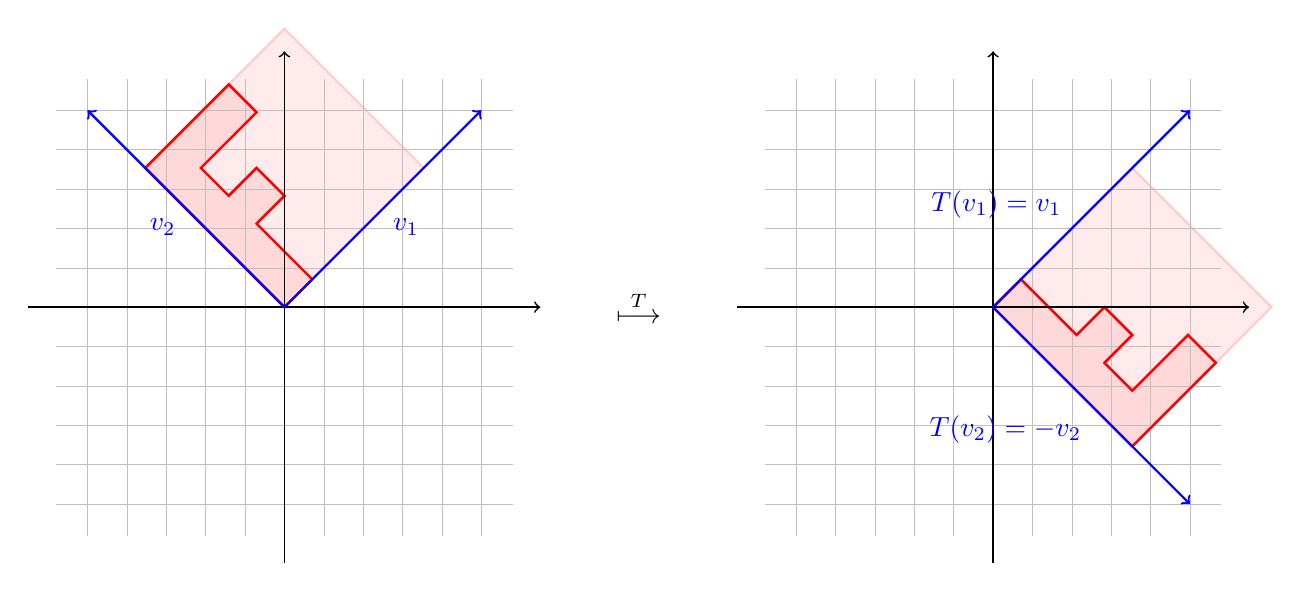
\begin{tikzpicture}
      \begin{scope}[scale=0.5]
        \draw[red!20,thick,fill=red!8,rotate=45]
        (0,0) -- (0,5) -- (5,5) -- (5,0) -- cycle;
        \draw[red,thick,fill=red!15,rotate=45]
        (0,0) -- (0,5) -- (3,5) -- (3,4) -- (1,4) --
        (1,3) -- (2,3) -- (2,2) -- (1,2) -- (1,0) -- cycle;
        \draw[step=1cm, gray!50, very thin] (-5.8,-5.8) grid (5.8,5.8);
        \draw[red,thick,rotate=45]
        (0,0) -- (0,5) -- (3,5) -- (3,4) -- (1,4) --
        (1,3) -- (2,3) -- (2,2) -- (1,2) -- (1,0) -- cycle;
        \draw[semithick,->] (-6.5,0) -- (6.5,0);
        \draw[semithick,->] (0,-6.5) -- (0,6.5);
        \draw[blue,thick,->] (0,0) -- node[below right] {$\vect{v}_1$} (5,5);
        \draw[blue,thick,->] (0,0) -- node[below left] {$\vect{v}_2$} (-5,5);
      \end{scope}
      \begin{scope}[xshift=4.5cm]
        \path (0,0) node {$\stackrel{T}{\longmapsto}$};
      \end{scope}
      \begin{scope}[xshift=9cm,scale=0.5]
        \draw[red!20,thick,fill=red!8,rotate=45,yscale=-1]
        (0,0) -- (0,5) -- (5,5) -- (5,0) -- cycle;
        \draw[red,thick,fill=red!15,rotate=45,yscale=-1]
        (0,0) -- (0,5) -- (3,5) -- (3,4) -- (1,4) --
        (1,3) -- (2,3) -- (2,2) -- (1,2) -- (1,0) -- cycle;
        \draw[step=1cm, gray!50, very thin] (-5.8,-5.8) grid (5.8,5.8);
        \draw[red,thick,rotate=45,yscale=-1]
        (0,0) -- (0,5) -- (3,5) -- (3,4) -- (1,4) --
        (1,3) -- (2,3) -- (2,2) -- (1,2) -- (1,0) -- cycle;
        \draw[semithick,->] (-6.5,0) -- (6.5,0);
        \draw[semithick,->] (0,-6.5) -- (0,6.5);
        \draw[blue,thick,->,cm={0,1,1,0,(0,0)}] (0,0) --
        node[above left,pos=0.4]
        {$T(\vect{v}_1) = \vect{v}_1$}
        (5,5);
        \draw[blue,thick,->,cm={0,1,1,0,(0,0)}] (0,0) --
        node[below left,pos=0.5]
        {$T(\vect{v}_2) = -\vect{v}_2$}
        (-5,5);
      \end{scope}
    \end{tikzpicture}
  \end{center}
  We see that this linear transformation is a reflection about the
  vector $\vect{v}_1$.
\end{solution}

\begin{example}
  Visualize the linear transformation $T:\R^2\to\R^2$ that is
  described by the matrix
  \begin{equation*}
    A = \begin{mymatrix}{rr}
      -2 & 3 \\
      0 &  1 \\
    \end{mymatrix}
  \end{equation*}
  by considering the eigenvectors and eigenvalues.
\end{example}

\begin{solution}
  The characteristic polynomial is $(-2-\lambda)(1-\lambda)$, and
  therefore, the eigenvalues are $\lambda_1=-2$ and $\lambda_2=1$.
  We find that the corresponding basic eigenvectors are
  \begin{equation*}
    \vect{v}_1 = \begin{mymatrix}{r} 1 \\ 0 \end{mymatrix}
    \quad\mbox{and}\quad
    \vect{v}_2 = \begin{mymatrix}{r} 1 \\ 1 \end{mymatrix},
  \end{equation*}
  respectively. We get the following before-and-after picture:
  \begin{center}
    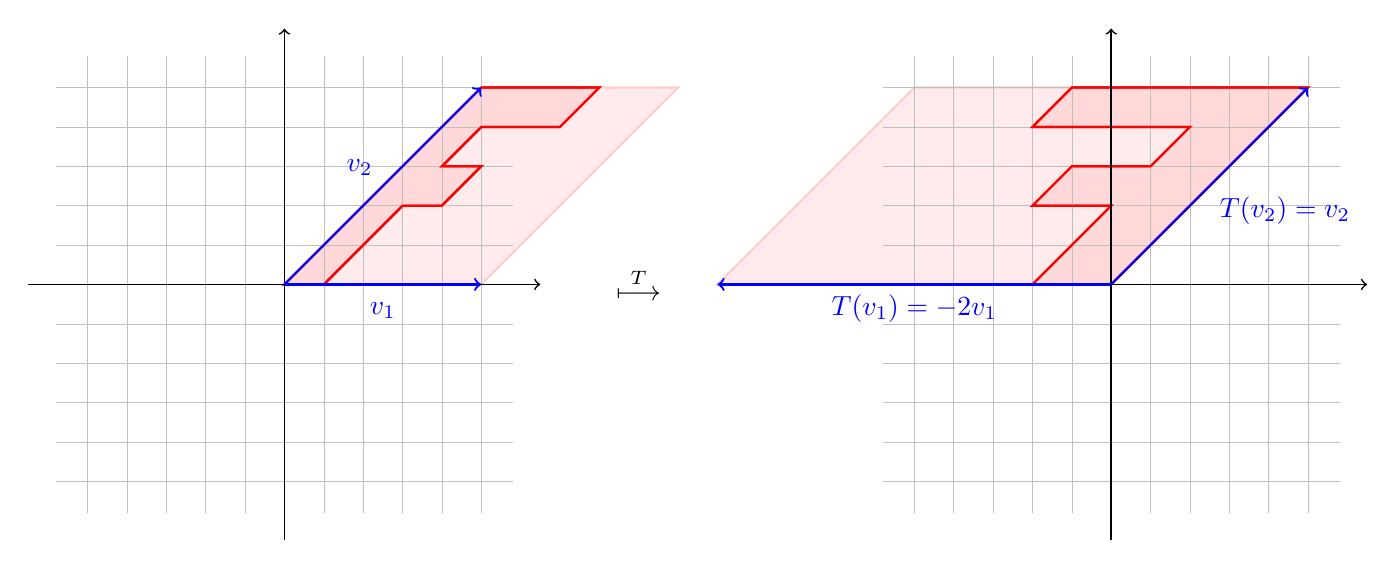
\begin{tikzpicture}
      \begin{scope}[scale=0.5]
        \draw[red!20,thick,fill=red!8,cm={1,0,1,1,(0,0)}]
        (0,0) -- (0,5) -- (5,5) -- (5,0) -- cycle;
        \draw[red,thick,fill=red!15,cm={1,0,1,1,(0,0)}]
        (0,0) -- (0,5) -- (3,5) -- (3,4) -- (1,4) --
        (1,3) -- (2,3) -- (2,2) -- (1,2) -- (1,0) -- cycle;
        \draw[step=1cm, gray!50, very thin] (-5.8,-5.8) grid (5.8,5.8);
        \draw[red,thick,cm={1,0,1,1,(0,0)}]
        (0,0) -- (0,5) -- (3,5) -- (3,4) -- (1,4) --
        (1,3) -- (2,3) -- (2,2) -- (1,2) -- (1,0) -- cycle;
        \draw[semithick,->] (-6.5,0) -- (6.5,0);
        \draw[semithick,->] (0,-6.5) -- (0,6.5);
        \draw[blue,thick,->,cm={1,0,1,1,(0,0)}] (0,0) -- node[below,yshift=-.1cm] {$\vect{v}_1$} (5,0);
        \draw[blue,thick,->,cm={1,0,1,1,(0,0)}] (0,0) -- node[above left] {$\vect{v}_2$} (0,5);
      \end{scope}
      \begin{scope}[xshift=4.5cm]
        \path (0,0) node {$\stackrel{T}{\longmapsto}$};
      \end{scope}
      \begin{scope}[xshift=10.5cm,scale=0.5]
        \draw[red!20,thick,fill=red!8,cm={-2,0,1,1,(0,0)}]
        (0,0) -- (0,5) -- (5,5) -- (5,0) -- cycle;
        \draw[red,thick,fill=red!15,cm={-2,0,1,1,(0,0)}]
        (0,0) -- (0,5) -- (3,5) -- (3,4) -- (1,4) --
        (1,3) -- (2,3) -- (2,2) -- (1,2) -- (1,0) -- cycle;
        \draw[step=1cm, gray!50, very thin] (-5.8,-5.8) grid (5.8,5.8);
        \draw[red,thick,cm={-2,0,1,1,(0,0)}]
        (0,0) -- (0,5) -- (3,5) -- (3,4) -- (1,4) --
        (1,3) -- (2,3) -- (2,2) -- (1,2) -- (1,0) -- cycle;
        \draw[semithick,->] (-6.5,0) -- (6.5,0);
        \draw[semithick,->] (0,-6.5) -- (0,6.5);
        \draw[blue,thick,->,cm={-2,0,1,1,(0,0)}] (0,0) --
        node[below]
        {$T(\vect{v}_1) = -2\vect{v}_1$}
        (5,0);
        \draw[blue,thick,->,cm={-2,0,1,1,(0,0)}] (0,0) --
        node[below right,pos=0.5]
        {$T(\vect{v}_2) = \vect{v}_2$}
        (0,5);
      \end{scope}
    \end{tikzpicture}
  \end{center}
  This particular linear transformation keeps the vector $\vect{v}_2$
  fixed, while scaling by a factor of $-2$ in the direction of
  $\vect{v}_1$. It could be described as a kind of slanted reflection
  with scaling.
\end{solution}
